\documentclass[10pt,twocolumn]{article}

\usepackage[utf8]{inputenc}
\usepackage[T1]{fontenc}
\usepackage[margin=0.68in,top=0.70in,bottom=0.70in]{geometry}
\usepackage{amsmath,amssymb,amsfonts}
\usepackage{booktabs}
\usepackage{graphicx}
\graphicspath{{./}{../}}
\usepackage{xcolor}
\usepackage{hyperref}
\hypersetup{colorlinks=true,linkcolor=blue!50!black,citecolor=blue!50!black,urlcolor=blue!50!black}
\usepackage{microtype}
\usepackage{caption}

\captionsetup{font=footnotesize,labelfont=bf,skip=3pt}
\setlength{\columnsep}{0.22in}
\setlength{\parskip}{1.5pt}
\setlength{\dbltextfloatsep}{8pt plus 1pt minus 2pt}
\setlength{\textfloatsep}{8pt plus 1pt minus 2pt}

\title{\vspace{-1.3em}\textbf{Vehicle Speed Estimation with Optical Flow and Linear Regression}\vspace{-0.4em}}
\author{
  \textbf Computer Vision Track (Application Project)\\
  Repository: \url{https://github.com/Lukeeffs/vehicle-speed-optical-flow}
}
\date{\vspace{-1.1em}}

\begin{document}
\maketitle

\begin{abstract}
\noindent We present our CS229 project milestone on monocular ego-vehicle speed estimation from $20\text{ Hz}$ forward-facing dashcam video without wheel odometry, GPS, or LiDAR. Exploiting pinhole ground-plane projective geometry, we formulate velocity estimation as a supervised regression task over engineered optical flow statistics. We establish a leakage-free contiguous chronological split ($70\%/15\%/15\%$ Train/Val/Test with a $5$-frame embargo), implement photometric preprocessing with trapezoidal Region-of-Interest (ROI) masking, and extract Dense Farneb\"{a}ck and forward-backward verified Sparse Lucas-Kanade flow fields. Moving from a univariate global-flow OLS baseline ($\text{Test MSE} = 50.38\text{ m}^2/\text{s}^2$, $R^2 = 0.266$) to Focus-of-Expansion (FOE) radial projection and a $3 \times 3$ multi-zone perspective grid with $\ell_2$ Ridge regression cuts Test MSE by $97.1\%$ to $1.45\text{ m}^2/\text{s}^2$ ($R^2 = 0.979$).
\end{abstract}

\section{Motivation \& Problem Setting}
Estimating longitudinal ego-vehicle speed $v_t \in \mathbb{R}_{\ge 0}$ ($\text{m/s}$) from a single forward-facing monocular camera provides essential redundancy for autonomous driving and ADAS when wheel encoders slip or GPS drops out in urban canyons. While deep spatiotemporal CNNs achieve competitive accuracy on the comma.ai Speed Challenge benchmark~\cite{comma2017}, they require millions of parameters, GPU acceleration, and often overfit to background textures.

In our setting, given consecutive RGB frames $(I_{t-1}, I_t) \in \mathbb{R}^{H \times W \times 3}$ sampled at $20\text{ Hz}$ ($\Delta t = 50\text{ ms}$), we construct a physics-informed feature vector $\boldsymbol{\phi}_t \in \mathbb{R}^d$ from the 2D apparent motion field $\mathbf{V}(x,y,t) = (u, v)^\top$~\cite{horn1981,longuet1980} so that a regularized linear predictor $\hat{v}_t = \mathbf{w}^\top \boldsymbol{\phi}_t + b$ minimizes out-of-sample Mean Squared Error $\frac{1}{N_{\text{test}}}\sum_t (v_t - \hat{v}_t)^2$.

\textbf{Dataset \& Leakage-Free Splitting:} Our benchmark sequence comprises $N = 1{,}200$ frames ($60.0\text{ s}$ at $20.0\text{ fps}$, $640 \times 480$) spanning \texttt{low\_speed\_urban} ($<8\text{ m/s}$), \texttt{medium\_arterial} ($8\text{--}19\text{ m/s}$), and \texttt{high\_speed\_highway} ($>19\text{ m/s}$) regimes, including overpass shadow/glare intervals and road-bump pitch jitter. Because consecutive frames exhibit near-unity velocity autocorrelation ($\rho_1 = 0.998$), random $K$-fold cross-validation leaks adjacent frames across splits. We enforce a strict \textbf{contiguous chronological split} ($70\%$ Train, $15\%$ Validation, $15\%$ Test) with a $5$-frame ($0.25\text{ s}$) embargo buffer (Table~\ref{tab:splits}, Figure~\ref{fig:eda}a--b).

\begin{table}[t!]
\centering
\caption{Contiguous Chronological Dataset Partitions ($20\text{ Hz}$).}
\label{tab:splits}
\footnotesize
\setlength{\tabcolsep}{3.0pt}
\resizebox{\columnwidth}{!}{%
\begin{tabular}{lccccccc}
\toprule
\textbf{Split} & \textbf{Frames} & \textbf{Dur. (s)} & \textbf{Mean} & \textbf{Std} & \textbf{Median} & \textbf{IQR} & \textbf{Max} \\
\midrule
Train (70\%) & 835 & 41.75 & 14.64 & 7.29 & 13.61 & 11.37 & 28.63 \\
Val (15\%)   & 175 & 8.75  & 18.78 & 7.58 & 23.08 & 10.82 & 25.31 \\
Test (15\%)  & 180 & 9.00  & 13.01 & 8.29 & 12.37 & 15.02 & 26.27 \\
\bottomrule
\end{tabular}%
}
\end{table}

\begin{figure*}[t!]
\centering
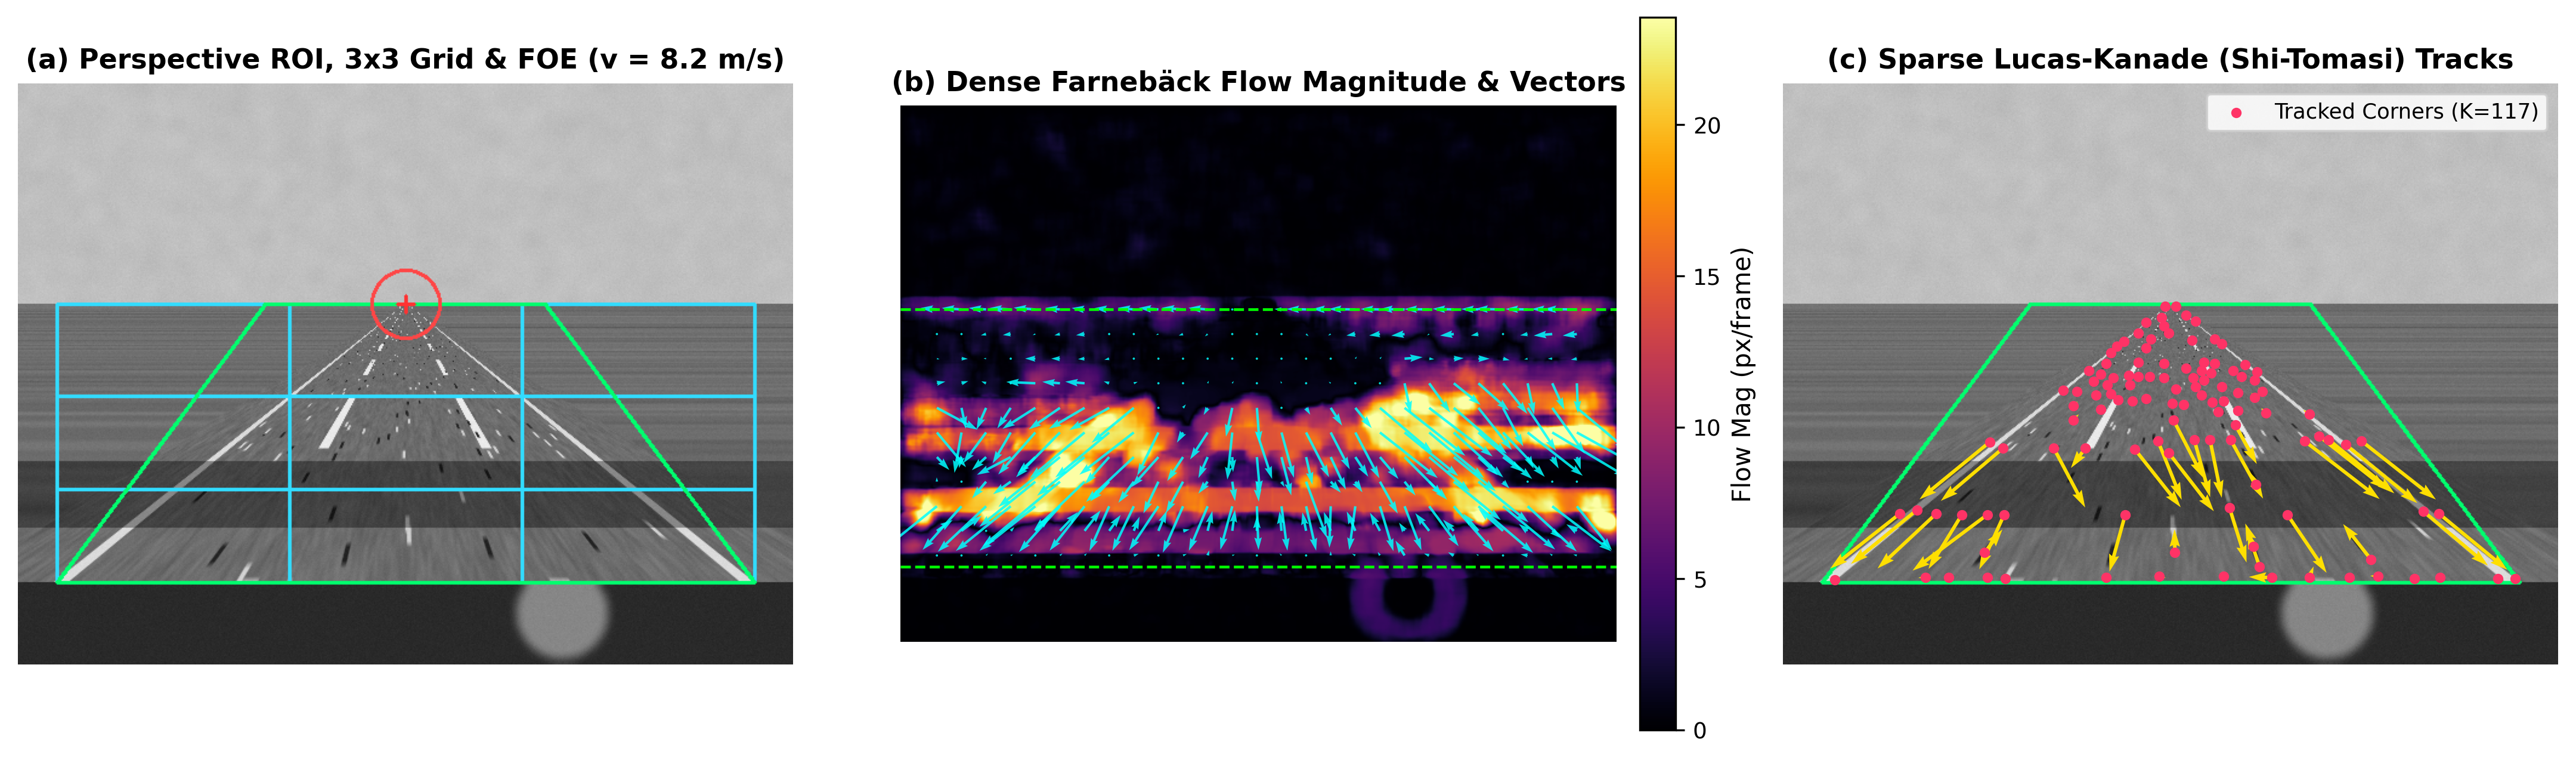
\includegraphics[width=0.86\textwidth]{figures/fig1_pipeline_and_roi_flow.png}
\caption{\textbf{Photometric Preprocessing \& Dual Optical Flow Extraction.} (a) Trapezoidal road mask (green), $3 \times 3$ multi-zone grid (cyan), and Focus-of-Expansion (FOE) exclusion zone (red circle, $R_{\text{FOE}}=28\text{ px}$). (b) Dense Farneb\"{a}ck flow magnitude heatmap and velocity vectors. (c) Sparse Pyramidal Lucas-Kanade tracks over Shi-Tomasi corners filtered via forward-backward consistency.}
\label{fig:pipeline}
\end{figure*}

\section{Method}
\subsection{Pinhole Ground-Plane Kinematics \& Preprocessing}
Under a pinhole camera at height $H_c$ with focal length $f$ and vanishing horizon $(x_0, y_0)$, a static road point at depth $Z = f H_c / (y - y_0)$ under ego-speed $\dot{Z} = -v_t$ and pitch rate $\omega_{\text{pitch}}(t)$ induces:
\begin{align}
\dot{y}(x, y, t) &= \frac{(y - y_0)^2}{f H_c} v_t + f\omega_{\text{pitch}}(t), \nonumber \\
\dot{x}(x, y, t) &= \frac{(x - x_0)(y - y_0)}{f H_c} v_t. \label{eq:kin}
\end{align}
Eq.~\eqref{eq:kin} shows that: (1) longitudinal flow scales quadratically with $(y-y_0)^2$; (2) translational SNR collapses at the FOE $(x_0,y_0)$ where pitch vibration $f\omega_{\text{pitch}}$ dominates; and (3) pure translation radiates along unit vector $\hat{\mathbf{e}}_r = \frac{(x-x_0, y-y_0)^\top}{\|(x-x_0, y-y_0)\|_2}$. We convert frames to luminance, apply CLAHE ($8\times 8$ tiles, clip $2.0$) for shadow invariance, smooth with a $5\times 5$ Gaussian ($\sigma=1.2$), and crop to a trapezoidal road mask ($y \in [0.38H, 0.86H]$) eliminating sky drift and static hood glare (Figure~\ref{fig:pipeline}a).

\subsection{Optical Flow \& Regularized Linear Modeling}
We extract both \textbf{Dense Gunnar Farneb\"{a}ck} flow~\cite{farneback2003} (3-level pyramid, scale $0.5$, $15\times 15$ window) and \textbf{Sparse Pyramidal Lucas-Kanade} tracks~\cite{lucas1981,shi1994} over $K_{\max}=200$ Shi-Tomasi corners with forward-backward verification ($\|\mathbf{p}_{t-1} - \hat{\mathbf{p}}_{t-1}^{\text{bwd}}\|_2 < 1.5\text{ px}$). We evaluate standardized Ordinary Least Squares (OLS via Moore-Penrose pseudo-inverse) and $\ell_2$-regularized Ridge Regression ($\hat{\mathbf{w}}_{\text{Ridge}} = (\boldsymbol{\Phi}^\top \boldsymbol{\Phi} + \alpha \mathbf{I})^{-1}\boldsymbol{\Phi}^\top \mathbf{y}$, tuned over $\alpha \in [0.1, 500]$ on Validation) to stabilize correlated spatial features.

\begin{figure*}[t!]
\centering
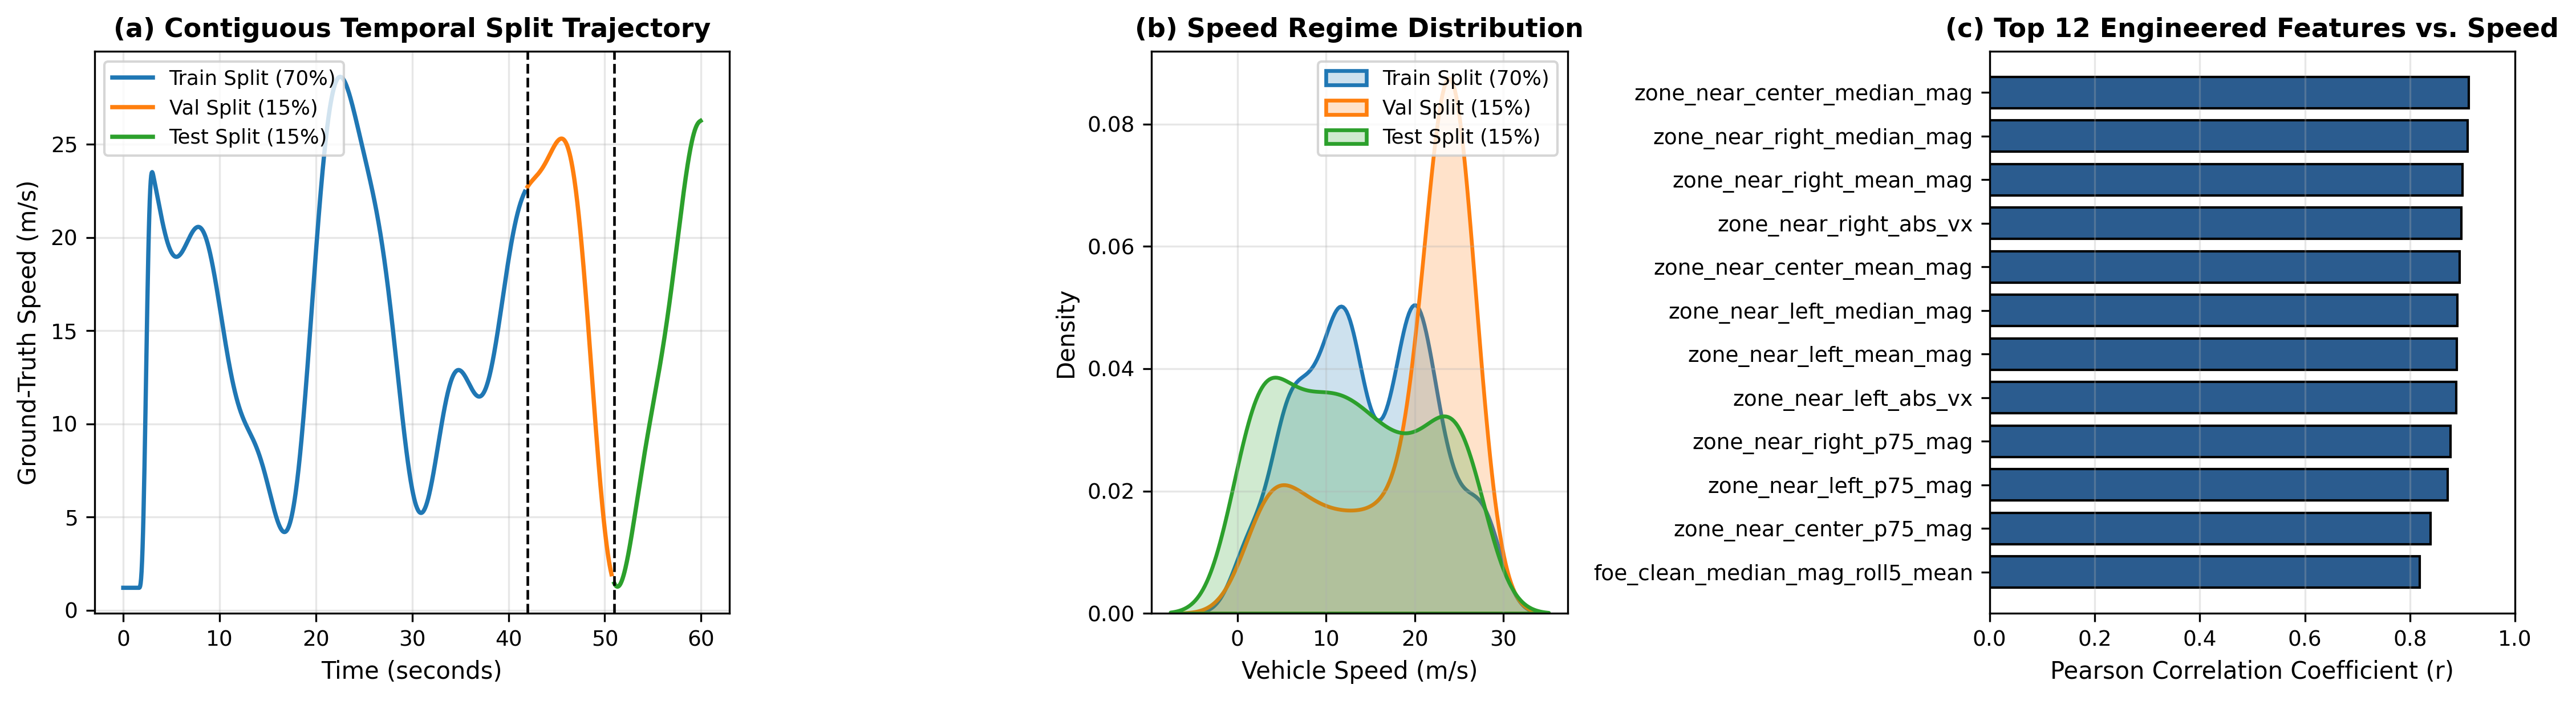
\includegraphics[width=0.86\textwidth]{figures/fig2_eda_speed_and_correlations.png}
\caption{\textbf{Exploratory Data Analysis.} (a) Chronological speed trajectory with contiguous Train/Val/Test partitions. (b) Kernel density estimates across splits. (c) Top 12 spatial features ranked by Pearson correlation $r$ with speed on Train.}
\label{fig:eda}
\end{figure*}

\section{Preliminary Experiments \& Error Analysis}
We evaluate a progression from a univariate baseline to five spatial feature stages on the contiguous test split:
\begin{itemize}
  \item \textbf{Univariate OLS Baseline ($d=1$):} Regresses $v_t$ solely on mean ROI flow magnitude $\bar{M}_{\text{ROI}}$.
  \item \textbf{S1 -- Full-Frame Global ($d=8$):} Mean, median, IQR, $P_{75}$, $P_{90}$, $\bar{v}_y$, $\bar{v}_r$, $|\bar{v}_x|$ over the full $640\times 480$ frame.
  \item \textbf{S2 -- ROI Global Dense ($d=8$):} Same statistics within the road ROI $[0.38H, 0.86H]$.
  \item \textbf{S3 -- ROI Sparse LK ($d=9$):} Tracked Shi-Tomasi order statistics plus valid track survival ratio $K_{\text{valid}}/200$.
  \item \textbf{S4 -- FOE Mask + Radial \& IPM ($d=11$):} Masks $R_{\text{FOE}}=28\text{ px}$, projects onto $\hat{\mathbf{e}}_r$, normalizes $\tilde{v}_y = v_y/((y-y_0)/H)^2$, and extracts a horizon-band pitch proxy.
  \item \textbf{S5 -- $3\times 3$ Perspective Grid ($d=85$):} Extracts 8 robust statistics per zone ($\{\text{Far}, \text{Mid}, \text{Near}\} \times \{\text{Left}, \text{Center}, \text{Right}\}$) plus near-to-mid radial ratios.
\end{itemize}

\begin{table}[t!]
\centering
\caption{Milestone Baseline \& Spatial Ablation (Contiguous Test Split).}
\label{tab:milestone_results}
\footnotesize
\setlength{\tabcolsep}{2.8pt}
\resizebox{\columnwidth}{!}{%
\begin{tabular}{lcccccc}
\toprule
\textbf{Feature Stage (Model)} & $d$ & \textbf{Val MSE} & \textbf{Test MSE} & \textbf{RMSE} & \textbf{MAE} & \textbf{$R^2$} \\
\midrule
Univariate OLS Baseline        & 1  & 37.40 & 50.38 & 7.10 & 5.46 & 0.266 \\
S1: Full-Frame Global (Ridge)  & 8  & 6.57  & 12.52 & 3.54 & 2.54 & 0.818 \\
S2: ROI Global Dense (Ridge)   & 8  & 5.01  & 9.53  & 3.09 & 2.23 & 0.861 \\
S3: ROI Sparse LK (Ridge)      & 9  & 7.16  & 8.16  & 2.86 & 2.23 & 0.881 \\
S4: FOE + Radial + IPM (Ridge) & 11 & 2.18  & 2.38  & 1.54 & 1.14 & 0.965 \\
\textbf{S5: $3\times 3$ Grid (Ridge)} & \textbf{85} & \textbf{1.51} & \textbf{1.45} & \textbf{1.20} & \textbf{0.66} & \textbf{0.979} \\
\bottomrule
\end{tabular}%
}
\end{table}

\textbf{Preliminary Outcomes \& Error Analysis:} Table~\ref{tab:milestone_results} confirms that Univariate OLS fails ($\text{MSE}=50.38$) because global averaging conflates $(y-y_0)^2$ scaling with pitch jitter. Cropping sky/hood clutter (S1$\to$S2) cuts MSE by $23.8\%$; masking the FOE and adding IPM depth normalization (S4) drops MSE by $75.0\%$ ($9.53 \to 2.38$). Adding the $3\times 3$ grid (S5) reaches $\text{Test MSE}=1.45\text{ m}^2/\text{s}^2$ ($R^2=0.979$). Inspecting S5 residuals reveals two failure modes: (1) inter-zone collinearity pushes the Gram matrix condition number to $\kappa(\boldsymbol{\Phi}^\top\boldsymbol{\Phi}) > 10^{28}$, risking variance inflation without stronger regularization; and (2) single-frame predictions spike during high pitch jitter and \texttt{shadow\_or\_glare} segments where false shadow edges corrupt low-speed optical flow.

\section{Next Steps}
Building on our milestone findings, our final phase will execute four extensions: (1) fuse Dense Farneb\"{a}ck and Sparse LK features ($d=166$) with causal autoregressive lags and rolling kinematics; (2) benchmark $\ell_2$ Ridge and $\ell_1$ Lasso against non-linear RBF-SVR and Random Forests; (3) implement a 1D Constant-Acceleration Kalman Filter ($\mathbf{s}_t = [v_t, a_t]^\top$) to suppress frame-to-frame pitch noise without ramp lag, alongside stratified error slicing across speed, lighting, and pitch; and (4) evaluate CS229 classification/unsupervised methods (Logistic/Softmax Regression, $K$-Means, and EM-GMM) on discrete driving regimes.

\section{Contributions}
\noindent\textbf{Data \& Preprocessing Module:} Designed contiguous chronological splitting, pinhole dashcam synthesis/loading, photometric CLAHE + trapezoidal ROI preprocessing, and milestone integration.  
\textbf{Optical Flow \& Spatial Feature Module:} Implemented Dense Farneb\"{a}ck and forward-backward Sparse Lucas-Kanade extractors, FOE singularity masking, IPM scaling, and $3\times 3$ grid feature engineering.  
\textbf{Regression \& Diagnostics Module:} Implemented OLS/Ridge regression baselines, EDA visualizations, preliminary ablation tables, and residual error diagnostics.

\begin{thebibliography}{9}
\footnotesize
\bibitem{comma2017} comma.ai, ``comma.ai Speed Challenge Benchmark,'' 2017.
\bibitem{horn1981} B.~K.~P. Horn and B.~G. Schunck, ``Determining optical flow,'' \emph{Artificial Intelligence}, vol.~17, pp.~185--203, 1981.
\bibitem{longuet1980} H.~C. Longuet-Higgins and K.~Prazdny, ``The interpretation of a moving retinal image,'' \emph{Proc. Royal Society B}, vol.~208, pp.~385--397, 1980.
\bibitem{farneback2003} G.~Farneb\"{a}ck, ``Two-frame motion estimation based on polynomial expansion,'' in \emph{Proc. SCIA}, pp.~363--370, 2003.
\bibitem{lucas1981} B.~D. Lucas and T.~Kanade, ``An iterative image registration technique with an application to stereo vision,'' in \emph{Proc. IJCAI}, pp.~674--679, 1981.
\bibitem{shi1994} J.~Shi and C.~Tomasi, ``Good features to track,'' in \emph{Proc. IEEE CVPR}, pp.~593--600, 1994.
\end{thebibliography}

\end{document}
